\doublespacing
\chapter{BACKGROUND}

%add maxwell's eqauations and gprmax

\section{Introduction}
\hspace{0.5in}This chapter begins with the theory and applications of Ground Penetrating radar. Then, the necessary background and theory behind Neural Networks is briefly presented. Next, information is then extended with an in depth look at the principle and applications of generative models, which presents the basis for an introduction to Generative Adversarial networks where a large part of this thesis is contained. In support of this, the traditional means of evaluating generative models is explored. Finally, the principles of object identification and classification are presented to introduce the real time classification model. 

\section{Ground Penetrating Radar}\label{GPR Backround}
\hspace{0.5in}Ground Penetrating Radar (GPR) is one of the most widely used non-destructive techniques for subsurface imaging and detection of underground objects, such as landmines, utilities, and archaeological artifacts. In the GPR scanning process, an electromagnetic wave is propagated into the target subsurface medium through a transmitting antenna, and upon reflection of the underground object, returned to a receiving antenna. This process is carried out across the above-ground surface for multiple passes. As shown in Figure \ref{fig:image_compare} (a), a reflection signal scattering from the underground object can be received and recorded by the receive antenna. As the GPR antennas moves, the reflection signals from the buried object from a number of different angles are received with varying wave propagation distance and amplitude. As a result, the buried object exhibits the hyperbolic image feature in the radar image in Figure \ref{fig:image_compare} (b). For each hyperbola composition point, its time index and signal amplitude are determined by a number of object properties, including the depth, size, material type and object shape and the dielectric constant of burying medium. Each time the signal is sent into the material the reflected signal is measured as an A-scan signal, which is a 1-dimensional representation of the signal. A series of A-scans, when concatenated sequentially, form a 2-dimensional high resolution image called B-scan, as shown in figure \ref{fig:gpr_basics}. Within such B-scan images, underground objects appear particularly as hyperbolic-shaped signatures. The detection of buried objects can be therefore considered as the detection of reflected hyperbolas in GPR images.
\vspace{0.5\baselineskip}

\begin{figure}[H]
  \centering
  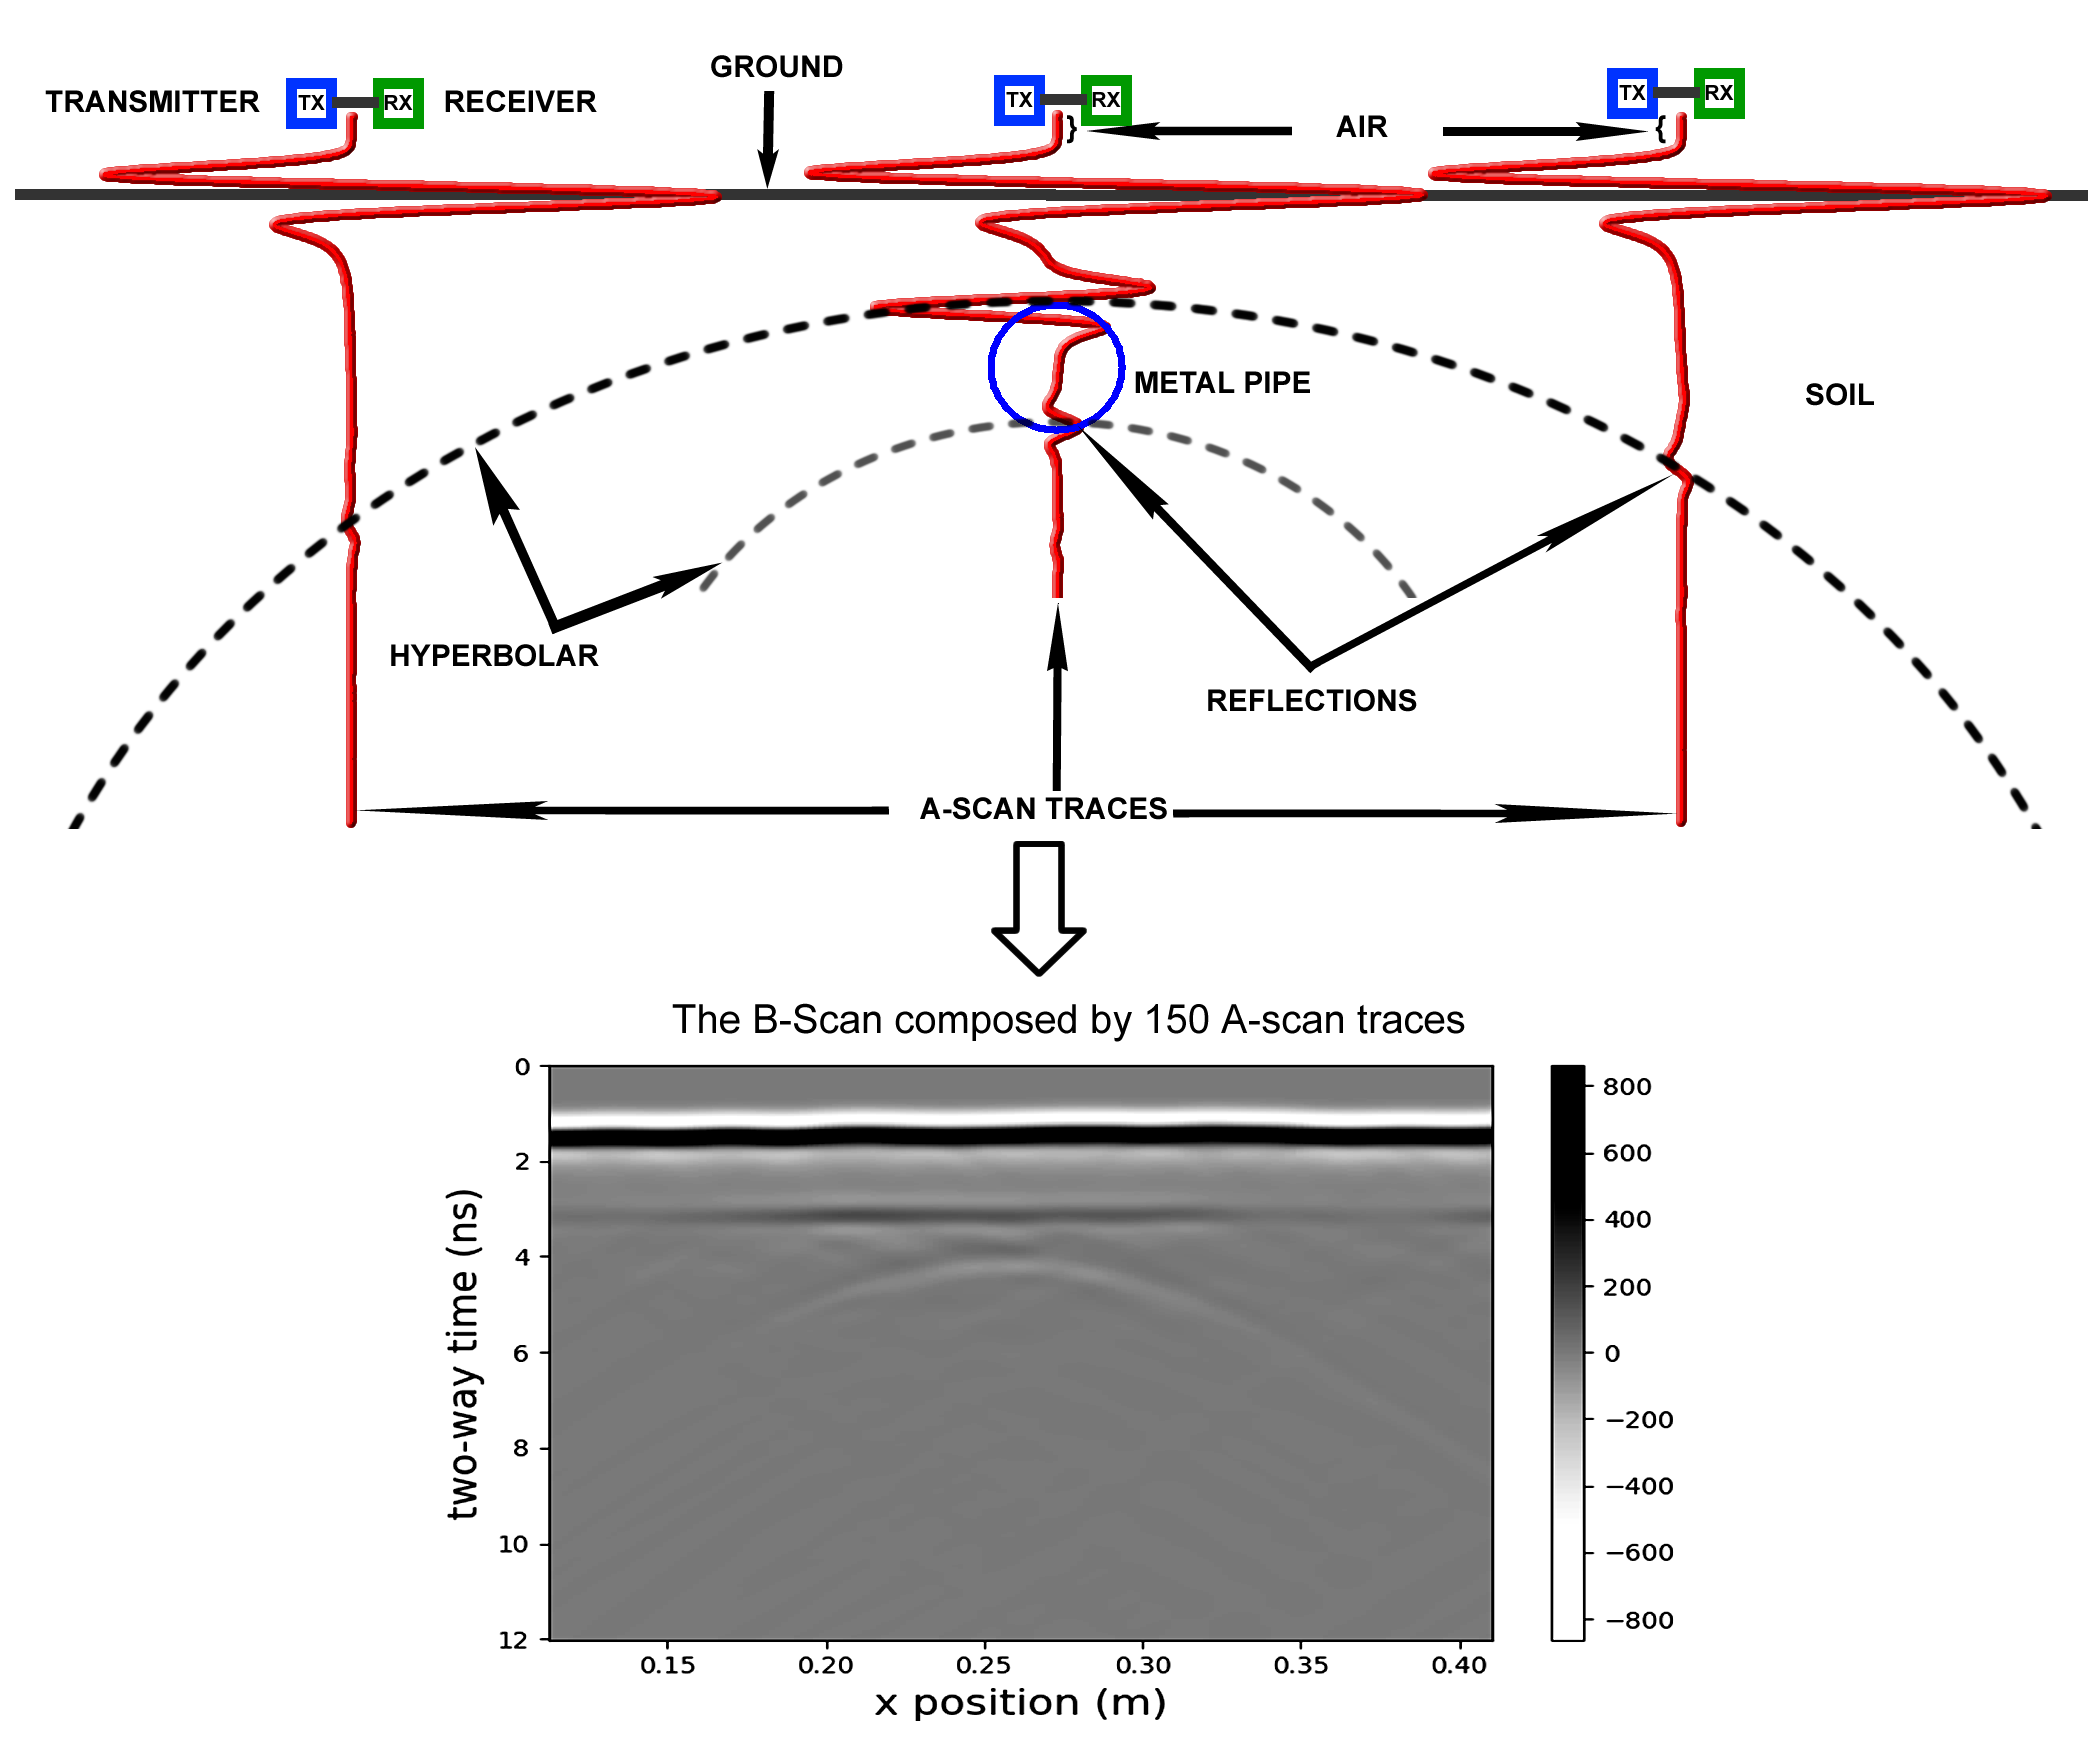
\includegraphics[width=1.0\linewidth]{figures/GPR_Original.png}
  \caption{\\Generator and Discriminator Architecture}
  \label{fig:gpr_basics}
\end{figure}

\subsection{Hands-on Collection}
 \hspace{0.5in}In March 2019, our team was able to walk alongside University of Vermont and get hands on experience in the collection of GPR data. Figure \ref{fig:mlk_collection} depicts a real B-scan in the location that it was taken. The collection process took several days to complete, and from this process we were able to obtained around 20 images. As one can see, collection in the field is a time consuming process. The collection time coupled with the amount of scans collected, is the primary reason GPR data are few.
 \vspace{0.5\baselineskip}

\begin{figure}[H]
    \centering
    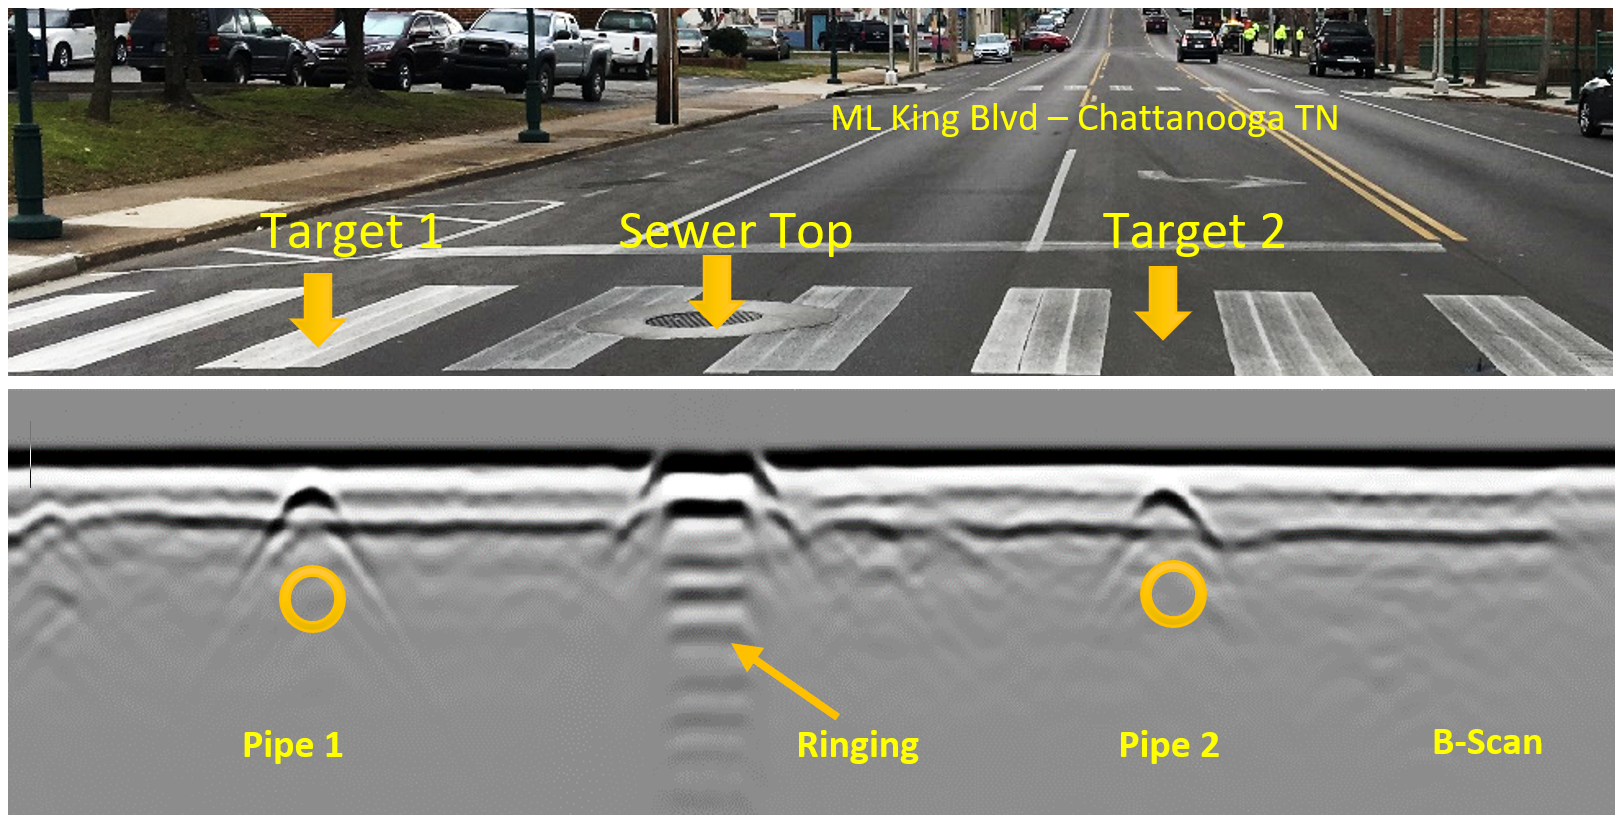
\includegraphics[width=\linewidth]{figures/mlk_collection.png}
    \caption{\\GPR Data Collection on MLK}
    \label{fig:mlk_collection}
\end{figure}


\subsection{B-scan Feature Processing}
\hspace{0.5in}B-scans, along with other features, are commonly analyzed to detect or identify subsurface objects. As an alternative to visual examination of B-scans by GPR technicians, machine learning techniques have been applied to analyze B-scans for object detection \cite{Zhang2016UndergroundOC, 6576024, 7860619, DBLP, 6009168}. By combining Hilbert transform and classic artificial neural network (ANN), the work in \cite{Zhang2016UndergroundOC} used amplitude and time from GPR A-Scan to detect the shape, material and depth of a buried object. Extracting a signal envelope, peak detection of envelope and depth of buried empty tube from A-Scan through analytic signal technique \cite{8075631}. Gilmore et.al \cite{7860619} extracted features using the Hu's seven invariant moments algorithm, and latter passed them through an ANN classifier \cite{6576024} to detect targets, however many false negatives were observed. While these techniques have been modestly effective, their performance is limited by the insufficient amount of real-world labeled GPR datasets for training the corresponding models or classifiers. To deal with the scarcity of GPR data, simulation-based methods  have been proposed to increase the availability of training data, but these methods fail to represent the full spectrum of features found in real GPR data. Therefore, classifiers trained on simulated B-scan images tend to perform poorly on real world B-scan images. A successful remedy is the combination of simulated and collected real-world GPR data in training \cite{DBLP}.
\vspace{0.5\baselineskip}

\begin{figure}[H]
    \centering
    \begin{subfigure}[b]{0.45\linewidth}
        
\includegraphics[width=\linewidth]{figures/before_preprocessing.png}
        \caption{\\Before}
    \end{subfigure}
    \begin{subfigure}[b]{0.45\linewidth}
        
\includegraphics[width=\linewidth]{figures/after_preprocessing.png}
        \caption{\\After}
    \end{subfigure}
    \caption{\\Before and After Pre-processing}
    \label{fig:preprocessing}
\end{figure}

\subsection{Frequency B-scan}
\vspace{0.5\baselineskip}

\begin{figure}[H]
    \centering
    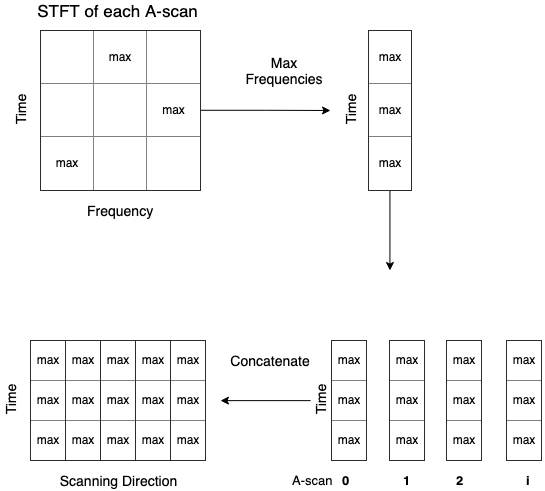
\includegraphics[width=0.8\linewidth]{figures/bscan_processing.png}
    
    \caption{\\Frequency B-scan Creation Process}
    \label{fig:bscan_processing}
\end{figure}

\vspace{0.5\baselineskip}
\begin{figure}[H]
    \centering
    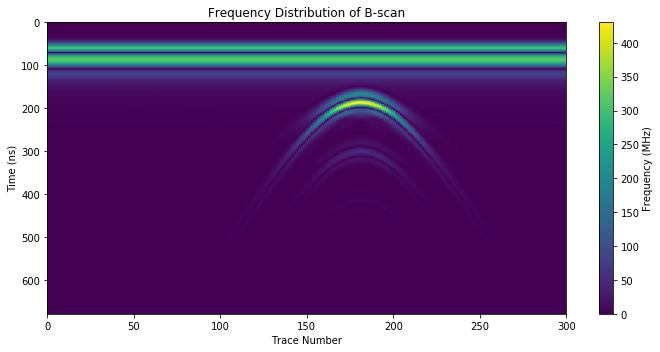
\includegraphics[width=0.6\linewidth]{figures/stft_b_scan_clean.png}
    
    \caption{\\Frequency B-scan}
    \label{fig:tf-bscan}
\end{figure}


\section{Neural Networks}
\hspace{0.5in}Neural Networks are a subset of machine learning algorithms that are inspired by neuron connections in the human brain. At the most basic level, the network consists of a single computational node that takes a vectored input, which is multiplied by a hidden weight, and transformed with a non-linearity to achieve an activated output. The idea is that the hidden weight can be optimized to produce a desired output. Networks may contain multiple nodes with many hidden layers. Some of the largest models can have hundreds of layers. For the purposes of this thesis, it is important to think of a neural network as an estimator of a probability distribution when given a conditional input. In fact, the activated output is commonly referred to as the posterior distribution. The name posterior simply indicates that it is the output distribution in respect of the prior, or to put succinctly, the inputs \cite{Goodfellow-et-al-2016}. This probabilistic approach will be very important in the next section, as it is a vital attribute of understanding how to measure the difference between distributions which is a core principle of generative models.

\section{Statistical Distance}
\hspace{0.5in}Statistical Distance is simply a measure of the difference between two distributions. In the context of machine learning, it is possible to train a model to reduce this difference. In the following subsections, we will discuss several ways to measure this difference, and how we can apply neural networks as a means of reducing this difference \cite{Goodfellow-et-al-2016}.

\subsection{Mean Squared Error}
\hspace{0.5in}Although not technically a statistical distance metric, we can think of \acrfull{mse} as a means of calculating how different the expected output is from the observed. Equation \ref{mse} is a generalized form of this concept. If we recall from the previous section, that a neural network can output a conditional distribution. From this output, we can calculate the difference between itself and the expected output. Furthermore, we can optimize the model to minimize this difference to coerce the output to be more similar to our expected output. In the next part, we will discuss another method of measuring difference between the observed and expected. A measure that is specifically designed for this problem \cite{Goodfellow-et-al-2016}.
\begin{center}
    \begin{equation}
    \label{mse}
        {MSE} ({\hat {\theta }})=\operatorname {E} _{\theta }\left[({\hat {\theta }}-\theta )^{2}\right]
    \end{equation}
\end{center}

\subsection{KL Divergence}
\hspace{0.5in}\acrfull{kld}\cite{kullback1951} can be thought of as a measure of the difference between two distributions $P$ and $Q$. Due to its asymmetric nature, \acrshort{kld} is not actually a true measurement of distance. However, the former conceptualization can remain for our purposes. An important feature of \acrshort{kld} is that it cannot be negative. Therefore, the minimum value is 0, at which, indicates that $P$ and $Q$ are the same distribution . Equation \ref{kl-divergence}, depicts the mathematical formula of \acrshort{kld}. Similar to \acrshort{mse}, this difference can be minimized by a neural network and has been successfully used as a loss function \cite{Goodfellow-et-al-2016}. However, the next measure is the most important in relation to this thesis.

\begin{center}
    \begin{equation}
    \label{kl-divergence}
       D_{\text{KL}}(P\parallel Q)=\sum _{x\in {\mathcal {X}}}P(x)\log \left({\frac {P(x)}{Q(x)}}\right)
    \end{equation}
\end{center}

\subsection{Wasserstein Distance}
\hspace{0.5in}A distribution can be described in terms of probability mass. If we know the shape of the mass, we can derive a method that moves mass in one distribution to match a target distribution. This is the idea of Optimal Transport Theory  and the Wasserstein metric is a solution to this problem. Commonly referred to as the earth mover's distance, the Wasserstein metric tells us how much mass we need to move to turn a given distribution into the target distribution. The task then becomes an issue of finding the proper function that transforms $p_r$ into $p_\Theta$ as shown in Equation \ref{wass-distance}. The importance in this, is that we can use a neural network to approximate the function, by training a model to minimize the Wasserstein distance. In approximating this function, we are able to take a prior distribution and transform it to closely match the target distribution. In the next section, we will see how this process can be applied to generate realistic data \cite{optimal-transport}.
\begin{center}
    \begin{equation}
    \label{wass-distance}
W(p_r, p_\theta) = \sup_{\lVert f \lVert_{L \leq 1}} \ \mathbb{E}_{s \sim p_r}[f(s)] - \mathbb{E}_{t \sim p_\theta}[f(t)]
    \end{equation}
\end{center}



\section{Generative Models}
\hspace{0.5in}Generative models are a subset of Neural Networks that enable the synthesis of realistic data. Research into this type of model has exploded over the last few years, mainly due to the types of problems that are able to be solved by them. For instance, generative models have been widely successful at generating realistic Speech, Music, Images, and Videos. The basis of this ability lies in the way neural networks are universal function approximators \cite{universal}. This allows a model to be fed inputs, learn the features of these inputs, and then produce outputs with the likeness of the input data. If we look at our inputs and outputs as probability distributions one can begin to see how it would be very important to be able to measure the differences in two probability distributions \cite{Goodfellow-et-al-2016}.


\section{Generative Adversarial Networks and Applications}
\hspace{0.5in}A Generative Adversarial Network (GAN) is a form of generative model, in which two separate models are entangled in a zero-sum game. The generative portion of the network is denoted as the generator $(G)$. The goal of the generator is to synthesize the most realistic posterior distribution. In opposition of the generator, the discriminator $(D)$, decides if the posterior distribution is legitimate, or a counterfeit. This process is carried out in tandem during training and can lead to instability \cite{GAN}. The input to the generator is a Gaussian noise vector $\mathcal{N}(0, 1)$. A transformation is applied to this vector, thus producing a posterior with equal dimensionality as the target distribution. Furthermore, this process is carried out by interpolation of the input vector through one or more deconvolution operations[citation]. The discriminator decomposes this output distribution into a binary probability through a sigmoid activation. The basics of this min-max game have changed very little since first proposal. 

\hspace{0.5in}\acrlong{gans} have received wide attention in the machine learning field for their potential to learn high-dimensional, complex real data distribution \cite{GAN, overview}. Specifically, they do not rely on any assumptions about the distribution and can generate real-like samples from latent space in a simple manner. This powerful property leads \acrshort{gans} to be used in many generative tasks to replicate the real-world rich content such as images, videos, speech, written language, and music \cite{overview}. There has been some work done on employing \acrshort{gans} for data augmentation in image classification using deep learning \cite{overview}. Furthermore, GAN can also be interpreted to measure the discrepancy between the generated data distribution and the real data distribution and then learn to reduce it. The discriminator is used to implicitly measure the discrepancy. Despite the advantage and theoretical support of GAN, many shortcomings have been found due to the practical issues and inability to implement the assumption in theory including the infinite capacity of the discriminator. There have been many attempts to solve these issues by changing the objective function, the architecture, etc. Moreover, the most recent additions to the adversarial framework have improved on many weak points in the original architecture. Wasserstein Loss has been used in GAN models to improve the stability of the adversarial game \cite{WGAN}. Moreover, this architecture can be further improved with the use of a gradient penalty term \cite{WGAN-GP}.


\section{Evaluation of Generative Models} \label{Evaluation of Generative Models}

\hspace{0.5in}Many generative architectures use Mean Opinion Score (MOS) or other qualitative metrics for model evaluation \cite{MOS}. This type of evaluation is readily available via Amazon Turkers or similar service that allows the general public to give an opinion. In our case, qualitative evaluation is unrealistic due to the requirement of domain expertise to detect the realistic nature of each synthesized \acrshort{gpr} signal. Moreover, we would like to stray away from qualitative evaluation and use a more quantitative method. In this work, we validate the quality of generated output by an improvement factor in the recognitive ability of our object identification model. It is important to note the parallels between this technique and the commonly used Inception Score \cite{inception}. However, with the lack of widespread availability of benchmark classifiers applied to this domain, we use another method.

\subsection{Optimization Paradox}\label{paradox}
%citation 
\hspace{0.5in}Evaluation of a generative models presents a very unique challenge in respect to other machine learning models. As we recently covered, the idea is that we train a generative model to match the distribution of the training set in the output distribution. In minimizing this distance, we approach the distribution of the training set. The challenge is that at some point during this process variation is lost. Traditionally, this would be called over-fitting. However, detecting over-fitting in a generative model presents an evaluation paradox. The main question is: how do you maximize the difference in distributions as a metric for detecting over-fitting, when the entire principle of optimization is to reduce this difference? As one can see, this presents a rather tricky environment for evaluating generative models. The answer to the perfect evaluation method for generative models is a hot topic, that at the time of this writing, does not have a definitive solution. However, in principle there exists an optimization point which retains qualitative realism, but also allows for maximum variability. It is finding this balance, that encompasses all major challenges of generative model evaluation.


\section{Object Recognition}
\hspace{0.5in}Object Recognition can be simply thought of as taking an image, and determining what object is in that image. In the case of this thesis, the objects are the different materials of underground cylinders. This is essentially a classification problem. One takes images with $N$ classes and trains a model to predict correctly each of these classes when presented with a new image. An important note is that these types of models are only able to predict supervised classes. For instance, if a model was trained to be a dog detector, and only saw images of dogs. The model would perform poorly on images of a zebra. Therefore, in the scope of this thesis, the only concern is for the model to predict a class out of the $N$ classes available during training. However, it would be possible to add an additional class $(N+1)$ to allow for a catch all that accepts anything that is not one of the supervised classes. This is beyond the scope of this work, because the only images being used are known to contain one of the classes of cylinders.


\section{Classification Evaluation Metrics}
\hspace{0.5in}As we saw in Section \ref{Evaluation of Generative Models}, evaluation is an important aspect of machine learning. Below, the most common evaluation metrics for classification are discussed. A precursor to this discussion, requires a few simple definitions. True Positive (TP), is the number of correct predictions. In contrast, True Negative (TN) is the number of correct predictions for the negative class. Furthermore, a False Negative (FN) is when the class was actually negative, but the model predicted the class to be positive. Likewise, a False Negative (FN), is a positive class that is classified as negative.

% Accuracy
\subsection{Accuracy}
\hspace{0.5in}By far, the most ubiquitous evaluation metric is accuracy. As depicted in \ref{accuracy}, accuracy is simply the fraction of true positives and true negatives over all of the observations. In Chapter \ref{results}, accuracy is reported. However, often it is more important to measure not only what the classifier gets right, but \textit{how} wrong the classifier is. The following equations will shed light on the incorrectness of the model and allow us to make inferences based on this information.
\begin{center}
    \begin{equation}
    \label{accuracy}
        \frac{TP+TN}{TP+TN+FP+FN}
    \end{equation}
\end{center}



% Precision
\subsection{Precision}
\hspace{0.5in}Precision is a measure of how often the model makes the correct prediction when looking at both correct predictions and predictions the model got wrong, when it was actually correct. Equation \ref{precision} is the equation for precision. It is the measure of True Positives over the total number of positive predictions.
\begin{center}
    \begin{equation}
    \label{precision}
        \frac{TP}{TP+FN}
    \end{equation}
\end{center}

% Recall
\subsection{Recall}
\hspace{0.5in}The next metric discussed is recall. To put plainly, this metric determines how often the model is right when giving a positive class prediction. Equation \ref{recall} shows that recall is defined as the number of True Positives over the total number of positive predictions. Now an even better evaluation metric would be the combination of precision and recall. F1-Score is exactly this metric.

\begin{center}
    \begin{equation}
    \label{recall}
       \frac{TP}{TP+FP}
    \end{equation}
\end{center}

% F1-score
\subsection{F1-Score}
\hspace{0.5in}F1-Score combines both precision and recall into a single metric. This allows for ease of optimization. When looking at maximizing only the F1-Score, by default, it is also possible to maximize precision and recall. This is arguably one of the best metrics for classification problems. From Equation \ref{f1-score}, it can be seen that F1-Score combines precision and recall to form a powerful evaluation metric.
\begin{center}
    \begin{equation}
    \label{f1-score}
        2 \cdot \frac{precision \cdot recall}{precision + recall}
    \end{equation}
\end{center}

